For TDI systems the cuts to form a Chv\'{a}tal closure are easy to characterise

\begin{thm} Let $P=\{x|Ax\leq b\}$ be a polyhedron with $Ax\leq b$ is TDI and $A$ integral. 

The Chv\'{a}tal closure is $P'=\{x|Ax\leq \lfloor b\rfloor\}$
\end{thm}

\begin{pr}[]For the case $P\neq \emptyset$. Let the Chv\'{a}tal closure be $C$

$C\subset \{x|Ax\leq \lfloor b\rfloor\}$. It is clear that rounding down the right sides constitutes a Gomory-Chv\'{a}tal cut. The closure may have some more, so it's smaller.

$\{x|Ax\leq \lfloor b\rfloor\} \subset C$. Let $y\geq 0$ such that $\trans y A$ is integral. We need to show 

\[\forall x: Ax\leq \lfloor b \rfloor: \trans y A \leq \lfloor \trans y b\rfloor\]

That means rounding down gives us the same solutions as we get by applying the definition of Chv\'{a}tal closure. To use TDIness we look at

\[\trans yb \stackrel{Ax\leq b}{\geq} \max \{\trans y Ax | Ax\leq b\} = \min \{\trans v b|v\geq 0, \trans v A = \trans y A\}\]

Since $\trans y A$ is integral and $Ax\leq b$ is TDI we know there is some integral optimal vector $v^*$ for the dual. We then get

\[\trans y A x =\trans {v^*} A x \stackrel{Ax\leq \lfloor b\rfloor}{\leq} \trans{v^*} \lfloor b\rfloor \leq \lfloor \trans{v^*} b\rfloor \leq \lfloor \trans y b\rfloor\]

Which proves the claim.
\qed \end{pr}

We know that every rational polyhedron (and every bounded polyhedron) has a minimal TDI system that defines it. We can then find the Chv\'{a}tal closure easily and get a new polyhedron, for which we can then again find a TDI description and repeat the procedure.

Unfortunately finding TDI descriptions is hard and the number of iterations can be arbitrarily large. The number of iterations of adding the Chv\'{a}tal closure until we get the integer hull is called the \emph{Chv\'{a}tal rank}.

\subsection{Gomory's cutting plane algorithm}

The idea is to run simplex and the look at the final tableau. Find some row with fractional result and round everything down. 

\[x_i + \sum_{j\in N} \bar a_{ij} x_j = \bar a_{i0} \quad \Rightarrow \quad x_i + \sum_{j\in N} \lfloor\bar a_{ij}\rfloor x_j = \lfloor\bar a_{i0}\rfloor\]

Add that as a new constraint and repeat. 

It is ok to round down the $\bar{a_{ij}}$ because $x\geq 0$ and rounding down makes everything smaller, so the inequality is still satisfied. Rounding down the $\bar a_{i0}$ is ok because that's just the Chv\'{a}tal cut.

The new constraint cuts off at least the optimal solution simplex found. This has the nice property that we don't add cuts in regions that aren't interesting to us.

\begin{Ex} Let the ILP we want to solve be
\begin{align*}
\min \quad& x_1-2x_2\\
s.t. \quad& -4x_1 +6x_2 \leq 9\\
& x_1+x_2 \leq 4
&x_1,x_2 \in \N
\end{align*}

The first solution we get with simplex is $x=(15/10,25/10)$. The interesting row in the tableau is

\[x_2+1/10 x_3 + 1/10x_4 = 25/10\]

We add the cut

\[x_2 \leq 2\]

With that constraint we get the solution $x=(3/4,2)$ with the following row in the tableau

\[x_1-1/4x_3 +6/4 x_5 = 3/4\]

We add the cut

\[x_1-x_3+x_5\leq 0\]

Because $x_3$ and $x_5$ are slack variables ($x_5$ is for the first cut), we can replace them 

\[x_5 = 2-x_2\qquad x_3=9+4x_1-6x_2\]

With these constraints we get an integral solution.
\end{Ex}

\begin{thm} Gomory's Algorithm terminates after a finite number of iterations, when it is using the lexicographic dual simplex.
\end{thm}

\marginpar{Lecture 19}
\subsection{Cuts for TSP}

Gomory's algorithm is a general method that works for any ILP. Creating the cuts doesn't assume anything about the combinatorial structure of the problem and hence often isn't optimal.

Here we want to show how to exploit the structure of a problem, the Travelling Salesman Problem, to find some cuts for the polyhedron.

We're given a graph $G=(V,E)$ and want to find a minimum cost tour. 

In the standard formulation that we've already seen we have a variable for each edge, indicating if the edge is in the tour.

\begin{align*}
\min \quad & \sum_{e\in E} x_e c_e\\
s.t.\quad & \sum_{e\in \delta(v)} x_e = 2 && \forall v\in V \quad \text{all nodes used}\\
	& \sum_{e\in E(S)} x_e \leq |S|-1 && \forall S\subset V, 2\leq |S| \leq |V-1| \quad \text{only one cycle}\\
	& x_e \in \{0,1\}
\end{align*}

As we already said this uses an exponential number of constraints, but we don't bother with that right now.

The cuts we will add use \emph{combs}

\begin{Def}[Comb] %pic
A comb with handle $H$ and teeth $T_1,\ldots T_k$ consists of node sets $H$ and $T_i$ such that $T_i \cap T_j = \emptyset$, $H\cap T_i\geq 1$ and $|T_i\backslash H |\geq 1$ and $k$ is $\geq 3$ and odd.
\end{Def}

\begin{figure}[hbt]
\begin{center}
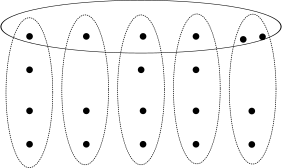
\includegraphics{./images/comb}
\end{center}
\caption{A comb in a graph}
\end{figure}

%If we have a comb in the graph no tour can exist in the graph.

\begin{thm} Let $c$ be a comb with handle $H$ and teeth $T_1,\ldots, T_k$. Then any tour satisfies the following inequality

\[\sum_{e\in E(H)} x_e +\sum_{i=1}^k\sum_{e\in E(T_i)} x_e \leq |H|+\sum_{i=1}^k(|T_i|-1)-\frac{k+1}{2}\]
\end{thm}

\begin{pr} To get the constraint from the theorem we take a linear combination of the constraints of the program and invoke the Chv\'{a}tal cut theorem.

Use

\begin{itemize}
\item Add the first constraint for all $v\in H$
\item Subtract the third inequality for (relaxed to $-x_e\leq 0$) for all $e\in \delta(H)\backslash X$ where $X$ are the edges that belong to a tooth
\item add the second constraint for all $T_i$
\item add the second constraint for all $T_i\backslash H$
\item add the second constraint for all $T_i \cap H$
\end{itemize}

The gets us the following equations

\begin{align*}
\sum_{v\in H}\sum_{e\in \delta(v)} x_e&=2|H|\\
-\sum_{v\in H} \sum_{e\in \delta(v) \backslash E(T_i)} x_e & \leq 0\\
+\sum_{i=1}^k \sum_{e\in E(T_i)} x_e &\leq \sum_{i=1}^k(|T_i|-1)\\
+\sum_{i=1}^k \sum_{e\in E(T_i\backslash H)} x_e &\leq \sum_{i=1}^k(|T_i\backslash H|-1)\\
+\sum_{i=1}^k \sum_{e\in E(T_i\cap H)} x_e &\leq \sum_{i=1}^k(|T_i\cap H|-1)\\
\end{align*}

Adding up the first two equations counts all the edges in the handle twice

\[2\sum_{e\in E(H)} x_e \leq 2|H|\]

The last two equations sum up to

\[\sum_{i=1}^k \sum_{e\in E(T_i)} x_e \leq \sum_{j=1}^k (|T_i|-1) -k\]

Summing up everything we get

\begin{align*}
2\sum_{e\in E(H)} x_e + 2\sum_{i=1}^k \sum_{e\in E(T_i)} x_e &\leq 2|H| + 2\sum_{j=1}^k (|T_i|-1) -k\\
\Leftrightarrow \sum_{e\in E(H)} x_e + \sum_{i=1}^k \sum_{e\in E(T_i)} x_e &\leq 2|H| + \sum_{j=1}^k (|T_i|-1) -\frac{k+1}{2}
\end{align*}

We replace $-k/2$ by $-(k+1)/2$ because $k$ is odd and we round everything down.
\qed \end{pr}

Unfortunately there are exponentially many comb cuts, and there is no polynomial algorithm to find one that is violated s.t. we might add it. There are however exponential time algorithms that find them and there are heuristic methods that sometimes find them.

So we can solve TSP by relaxing the LP. Usually we also drop the second constraint and allow more than one circle. We then try to find violated constraints. If we have more than one circle it's easy to find a violated constraint, else we have to find comb constraints either by the heuristic method or the exponential one. Should we be unable to find violated constraints although we don't have an integral solution yet, we need to use some other method like for example branch and bound.

\section{Branch and Bound}

With cutting plane algorithms we don't have any feasible solutions during the run of the algorithm, because we're solving relaxations all the time.

Branch and bound techniques actually work with feasible solutions that get improved iteratively. The approach is similar to divide-and conquer. We recursively partition the feasible region into sets and take the maximum (or the minimum) on it. That gives us a search tree of subproblems we need to solve. We use simplex or some other heuristic to find bounds on the optimal values such that we can cut off search paths that are not interesting.

There are some design choices we can make

\begin{itemize}
\item In what order to look at subproblems: DFS, BFS, Best-First, \ldots
\item How to compute bounds: LP relaxation, Lagragian relaxation (later), cutting planes
\end{itemize}

For general ILPs we can for example do the following: 

Use the LP relaxation for bounding. Branch by fixing components of the solution. For an optimal solution $x^*$ fix fractional values by adding constraints

\[x_i\leq  \lfloor x_i^*\rfloor \qquad x_i \geq \lceil x_i^* \rceil\]

\begin{Ex}[TSP] For the following relaxed formulation of the TSP

\begin{align*}
\min \quad & \sum_{i,j} c_{ij}x_{ij}\\
s.t. \quad & \sum_{j} x_{ij} = 1\\
	& \sum_{i} x_{ij} = 1\\
	& \sum_{ij\in S} x_{ij} \leq |S|-1 && S \subseteq \{1,\ldots,n\}, |S|\geq 2, |S| \leq |V|-1\\
	& x_{ij} \geq  0
\end{align*}

If we remove the constraint that forbids more than one circle we get the assignment problem (perfect matchings), which we can solve in polynomial time. We can use that as a bound for the TSP.

We branch by forbidding certain edges in the solution, i.e. we get some set of cycles from the relaxation, choose the shortest and create subproblems in which one of the edges on the cycle is fixed to 0.
\end{Ex}
